\begin{abcliste}
\abc Hephaistos fällt aus der Ruhe senkrecht hinunter. Als Kepler-Bahn ist das eine extrem schmale Ellipse (kleine Halbachse $b \to 0$, numerische Exzentrizität $\varepsilon \to 1$). Der Ausgangspunkt im Himmel ist das Apogäum, der erdfernste Punkt; der Erdmittelpunkt ist der Brennpunkt am anderen Ende der Ellipse. Der Fall entspricht der halben Ellipse vom Apogäum bis zur Erde.

\begin{center}
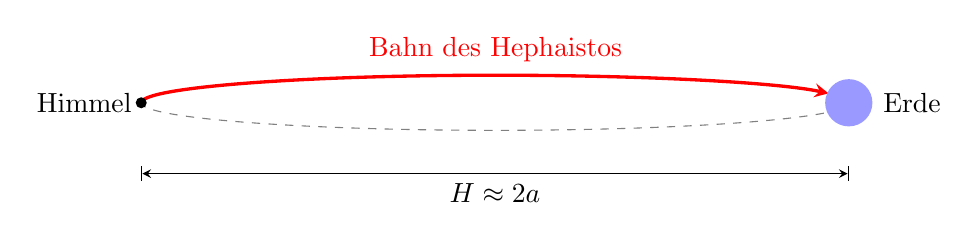
\begin{tikzpicture}[>=stealth]
 \draw[dashed, gray] (0,0) ellipse (4.5 and 0.35);
 \draw[very thick, red, ->] (-4.5,0) arc (180:20:4.5 and 0.35);
 \fill[blue!40] (4.486,0) circle (0.3);
 \node[right] at (4.8,0) {Erde};
 \fill (-4.5,0) circle (0.07) node[left] {Himmel};
 \node[red, above] at (0,0.4) {Bahn des Hephaistos};
 \draw[|<->|] (-4.5,-0.9) -- (4.486,-0.9) node[midway, below] {$H \approx 2a$};
\end{tikzpicture}

(nicht massstäblich)
\end{center}

\abc Für den Weg vom Apogäum bis zum Brennpunkt braucht ein Körper die halbe Umlaufzeit. Die Umlaufzeit der Ellipse ist deshalb
\begin{align}
 T &= \THeF = 2\cdot\tF = \THe
\end{align}
Der Mond umkreist ebenfalls die Erde, mit $T_\text{M} = \TMoO$ und $a_\text{M} = \aMoO$ (FoTaBe S.~210). Nach dem dritten Kepler'schen Gesetz, $a^3/T^2 = a_\text{M}^3/T_\text{M}^2$, ist die grosse Halbachse der Fallbahn
\begin{align}
 a &= \aHeF \\
   &= \aMo\cdot\left(\frac{\THe}{\TMo}\right)^{2/3} \\
   &= \aHe
\end{align}
Bei der extrem schmalen Ellipse liegt der Brennpunkt praktisch am Ende der grossen Achse. Der Himmel ist deshalb etwa die ganze grosse Achse vom Erdmittelpunkt entfernt:
\begin{align}
 H &= \HhF = \Hh \approx \result{\HhP{3}{2}}
\end{align}
Über der Erdoberfläche ($R_\text{E} = \RErdO$) sind das $H - R_\text{E} = \HueP{3}{2}$. Die grosse Halbachse $a$ ist ungefähr der Radius der geostationären Bahn, deren Umlaufzeit ebenfalls etwa einen Tag beträgt.
\end{abcliste}
